\documentclass[11pt]{amsart}
\usepackage[a4paper,margin=1in]{geometry}
\usepackage{amsmath,amssymb,amsthm}
\usepackage{graphicx}
\usepackage{booktabs}
\usepackage{tikz}
\usepackage[hidelinks]{hyperref}

\newtheorem{theorem}{Theorem}
\newtheorem{lemma}[theorem]{Lemma}
\theoremstyle{remark}
\newtheorem*{remark}{Remark}

\newcommand{\Z}{\mathbb Z}
\newcommand{\C}{\mathbb C}

\title{A periodic twelve-fold tiling by the Spectre}
\author{Vamshi Jandhyala}
\address{London, United Kingdom}
\email{vamshi.jandhyala@gmail.com}
\date{Preprint v1, 20 October 2026}
\subjclass[2020]{52C20, 05B45}
\keywords{Spectre, aperiodic monotile, multiple tiling, periodic tiling}

\begin{document}

\begin{abstract}
The Spectre of Smith, Myers, Kaplan and Goodman-Strauss tiles the plane by rotations and translations,
and every such tiling is non-periodic. Andrew Bayly asked whether it can tile the plane periodically if
each point is allowed to be covered $n$ times, for some $n>1$. It can: we give $54$ rotated and translated
copies of the Spectre whose translates by a lattice cover almost every point exactly $12$ times. The
proof is a finite check. The edges of the $54$ copies cancel in oppositely oriented pairs modulo the
lattice, so the covering number is constant, and comparing areas shows that the constant is $12$. For
the straight-edged Spectre the whole argument is formally verified in Lean.
\end{abstract}

\maketitle

\section{The question}

In 2023 Smith, Myers, Kaplan and Goodman-Strauss found a polygon, the Spectre, that tiles the plane using
rotations and translations but only non-periodically, and they showed that replacing its straight edges by
a suitable curve gives a strictly chiral tile with the same property~\cite{SMKG}. A tiling covers almost
every point once. In an \emph{$n$-fold tiling} almost every point lies in exactly $n$ tiles, overlaps being
allowed. Andrew Bayly asked on MathOverflow~\cite{MO} whether the Spectre admits a \emph{periodic}
$n$-fold tiling for some $n>1$, that is, a multiple tiling invariant under a lattice of translations.

\begin{theorem}\label{thm:main}
There is a periodic $12$-fold tiling of the plane by copies of the Spectre under rotations and
translations, with $54$ copies in each period cell. This holds for the straight-edged Spectre and for every
curved Spectre of the common-curve family.
\end{theorem}

The tiling uses no reflections and no two of its tiles coincide. Adding generic translates of the whole
configuration gives periodic tilings of every multiplicity $12m$. Whether some $1<n<12$ is possible is
open.

Periodic multiple tilings have been studied mainly for one tile moved by translations alone:
by convex or centrally symmetric polygons~\cite{Kol,GRS}, and, in the lattice $\Z^2$, by Greenfeld and
Tao, who proved the periodic tiling conjecture for multi-tilings of $\Z^2$: a finite set that
multi-tiles $\Z^2$ by translations also multi-tiles it periodically~\cite{GT}. The Spectre needs twelve rotations and its vertices lie in a
module of rank four, so neither line of work applies.

\section{The construction}

Let $\zeta=e^{\pi i/6}$. The straight-edged Spectre $\mathrm{Tile}(1,1)$ is the polygon with vertices
$p_0=0$ and $p_{i+1}=p_i+\zeta^{d_i}$ for $0\le i\le13$, where
\[
(d_0,\dots,d_{13})=(0,10,1,3,0,2,5,7,4,6,6,8,11,9).
\]
Its fourteen edges have unit length and directions that are multiples of $30^\circ$
(Figure~\ref{fig:tile}). Every vertex lies in $\Z[\zeta]$, which is a free abelian group with basis
$1,\zeta,\zeta^2,\zeta^3$, since $\zeta^4=\zeta^2-1$.

\begin{figure}[ht]
\centering
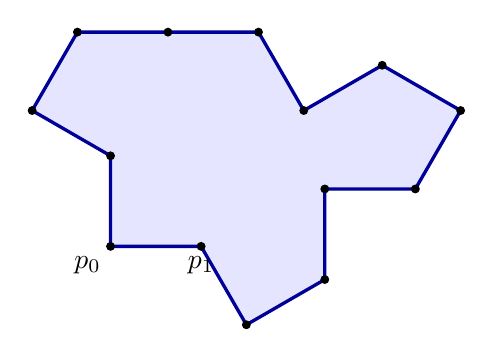
\begin{tikzpicture}[scale=1.15]
\fill[blue!10] (0.0000,0.0000) -- (1.0000,0.0000) -- (1.5000,-0.8660) -- (2.3660,-0.3660) -- (2.3660,0.6340) -- (3.3660,0.6340) -- (3.8660,1.5000) -- (3.0000,2.0000) -- (2.1340,1.5000) -- (1.6340,2.3660) -- (0.6340,2.3660) -- (-0.3660,2.3660) -- (-0.8660,1.5000) -- (0.0000,1.0000) -- cycle;
\draw[very thick,blue!60!black] (0.0000,0.0000) -- (1.0000,0.0000) -- (1.5000,-0.8660) -- (2.3660,-0.3660) -- (2.3660,0.6340) -- (3.3660,0.6340) -- (3.8660,1.5000) -- (3.0000,2.0000) -- (2.1340,1.5000) -- (1.6340,2.3660) -- (0.6340,2.3660) -- (-0.3660,2.3660) -- (-0.8660,1.5000) -- (0.0000,1.0000) -- cycle;
\foreach \p in {(0.0000,0.0000),(1.0000,0.0000),(1.5000,-0.8660),(2.3660,-0.3660),(2.3660,0.6340),(3.3660,0.6340),(3.8660,1.5000),(3.0000,2.0000),(2.1340,1.5000),(1.6340,2.3660),(0.6340,2.3660),(-0.3660,2.3660),(-0.8660,1.5000),(0.0000,1.0000)} \fill \p circle (1.4pt);
\node[below left] at (0,0) {$p_0$};
\node[below] at (1,0) {$p_1$};
\end{tikzpicture}
\caption{The straight-edged Spectre $\mathrm{Tile}(1,1)$, traced counterclockwise from $p_0=0$. In a curved
Spectre each edge is replaced by a copy of one curve, traversed forwards on even edges and backwards on odd
ones.}\label{fig:tile}
\end{figure}

A curved Spectre of the common-curve family~\cite[Lemma~2.1]{SMKG} replaces edge $i$ by
$p_i+\zeta^{d_i}\gamma(t)$ when $i$ is even and by $p_{i+1}+\zeta^{d_i+6}\gamma(1-t)$ when $i$ is odd, for a
fixed simple curve $\gamma$ from $0$ to $1$, chosen so that the boundary stays simple. Write $S$ for the
resulting tile. The regions added and removed along the edges cancel in pairs, so
\[
|S|=|\mathrm{Tile}(1,1)|=3+3\sqrt3 .
\]

Put
\[
a=\zeta^2+\zeta^3,\quad b=-2-\zeta-\zeta^3,\quad v=3+\zeta+2\zeta^2+3\zeta^3,\quad
w=-4-3\zeta+3\zeta^2+\zeta^3,
\]
and let $\Lambda=\Z v+\Z w$. The four vectors $a,b,v,w$ form a basis of $\Z[\zeta]$ (their determinant in
the basis $1,\zeta,\zeta^2,\zeta^3$ is $1$). The tiles are
\[
\zeta^rS+xa+yb+\lambda,\qquad \lambda\in\Lambda,
\]
for the $54$ triples $(r,y,x)$ of Table~\ref{tab:placements}.

\begin{table}[ht]
\centering
\begin{tabular}{rrl}
\toprule
$r$ & $y$ & values of $x$\\
\midrule
0 & 5 & $-2,-1,2,3$\\
1 & $-10$ & $-8$\\
2 & $-1$ & $-2,-1,\dots,5$\\
4 & $-10$ & $-5,-4,-3,-1,0,1$\\
4 & $-4$ & $-4,-3,0,1$\\
4 & 2 & $-3,1$\\
5 & 17 & $-1,3$\\
6 & $-13$ & $-9,-5$\\
6 & $-7$ & $-8,-7,-6,-4,-3,-2$\\
6 & $-1$ & $-3,1$\\
7 & 8 & $3,4,8$\\
8 & $-1$ & $-10,-9,\dots,-3$\\
10 & 2 & $-5,-1$\\
10 & 8 & $-5,-4,-1,0$\\
\bottomrule
\end{tabular}
\caption{The $54$ placements in one period cell: the tile $\zeta^rS+xa+yb$ for each listed $x$.}
\label{tab:placements}
\end{table}

\section{Why the covering number is constant}

For a point $z$ off all tile boundaries let $N(z)$ be the number of tiles containing it. It is invariant
under $\Lambda$, so it is a function on the torus $\C/\Lambda$.

\begin{lemma}\label{lem:pairs}
The $54\cdot14=756$ edges of the tiles in one period cell split into $378$ pairs. The two edges of a pair
are the same rotated copy of the edge curve, at the same position modulo $\Lambda$, traversed in opposite
directions.
\end{lemma}

The lemma is a finite check, and it can be done in integers. Every vertex of every tile lies in
$\Z[\zeta]$. The map $K\colon\Z^4\to\Z^2$ given by
\[
K=\begin{pmatrix}-2&3&0&1\\1&2&5&-5\end{pmatrix}
\]
in the basis $1,\zeta,\zeta^2,\zeta^3$ satisfies $Ka=(1,0)$, $Kb=(0,1)$ and $\ker K=\Lambda$, so $K$ reads off
the position of a point of $\Z[\zeta]$ modulo $\Lambda$. Record edge $i$ of the tile $(r,x,y)$ as
\[
\Bigl((r+d_i+6\varepsilon_i)\bmod 12,\ \ (x,y)+K\bigl(\zeta^rp_{i+\varepsilon_i}\bigr)\Bigr),
\qquad \varepsilon_i=i\bmod2,
\]
with sign $(-1)^i$. The first entry says which of the twelve rotated copies of the curve the edge is, and
the second where that copy starts modulo $\Lambda$; the sign says in which direction it is traversed. The
lemma says that the $378$ positive records and the $378$ negative records are the same multiset, and a
direct count confirms it.

\begin{proof}[Proof that $N$ is constant]
Off the tile boundaries, which form a null set, $N$ is locally constant. Crossing an edge of a tile from
its outside to its inside raises that tile's contribution by one. By Lemma~\ref{lem:pairs} every edge of the
period cell is matched, modulo $\Lambda$, by the same curve traversed the other way, which belongs to a tile
entered from the opposite side, so the two changes cancel and $N$ takes the same value on the two sides of
every edge. The torus is connected, so $N$ is constant almost everywhere.
\end{proof}

For the straight Spectre this argument is made precise in Lean through a triangulation: each tile is cut
into twelve triangles, the indicator of a triangle is a sum of signed ``shadows'' of its three edges, and the
$1944$ triangle edges cancel modulo $\Lambda$ (Section~\ref{sec:lean}). For a curved Spectre the step from
the cancelling records to the jump of $N$ across each edge uses the Jordan curve theorem for the edge curve.

\section{Why the constant is twelve}

In Cartesian coordinates,
\[
v=\Bigl(4+\tfrac{\sqrt3}{2},\ \tfrac72+\sqrt3\Bigr),\qquad
w=\Bigl(-\tfrac52-\tfrac{3\sqrt3}{2},\ -\tfrac12+\tfrac{3\sqrt3}{2}\Bigr),
\]
so a period cell has area $\det(v,w)=\tfrac{27}{2}(1+\sqrt3)$. Integrating the constant $N$ over a cell
counts each of the $54$ tiles once by area:
\[
N=\frac{54\,|S|}{\det(v,w)}=\frac{54\cdot3(1+\sqrt3)}{\tfrac{27}{2}(1+\sqrt3)}=12 .
\]
This proves Theorem~\ref{thm:main}. Figure~\ref{fig:cover} counts the tiles over a fine grid of points in four
period cells for one curved Spectre.

\begin{figure}[ht]
\centering
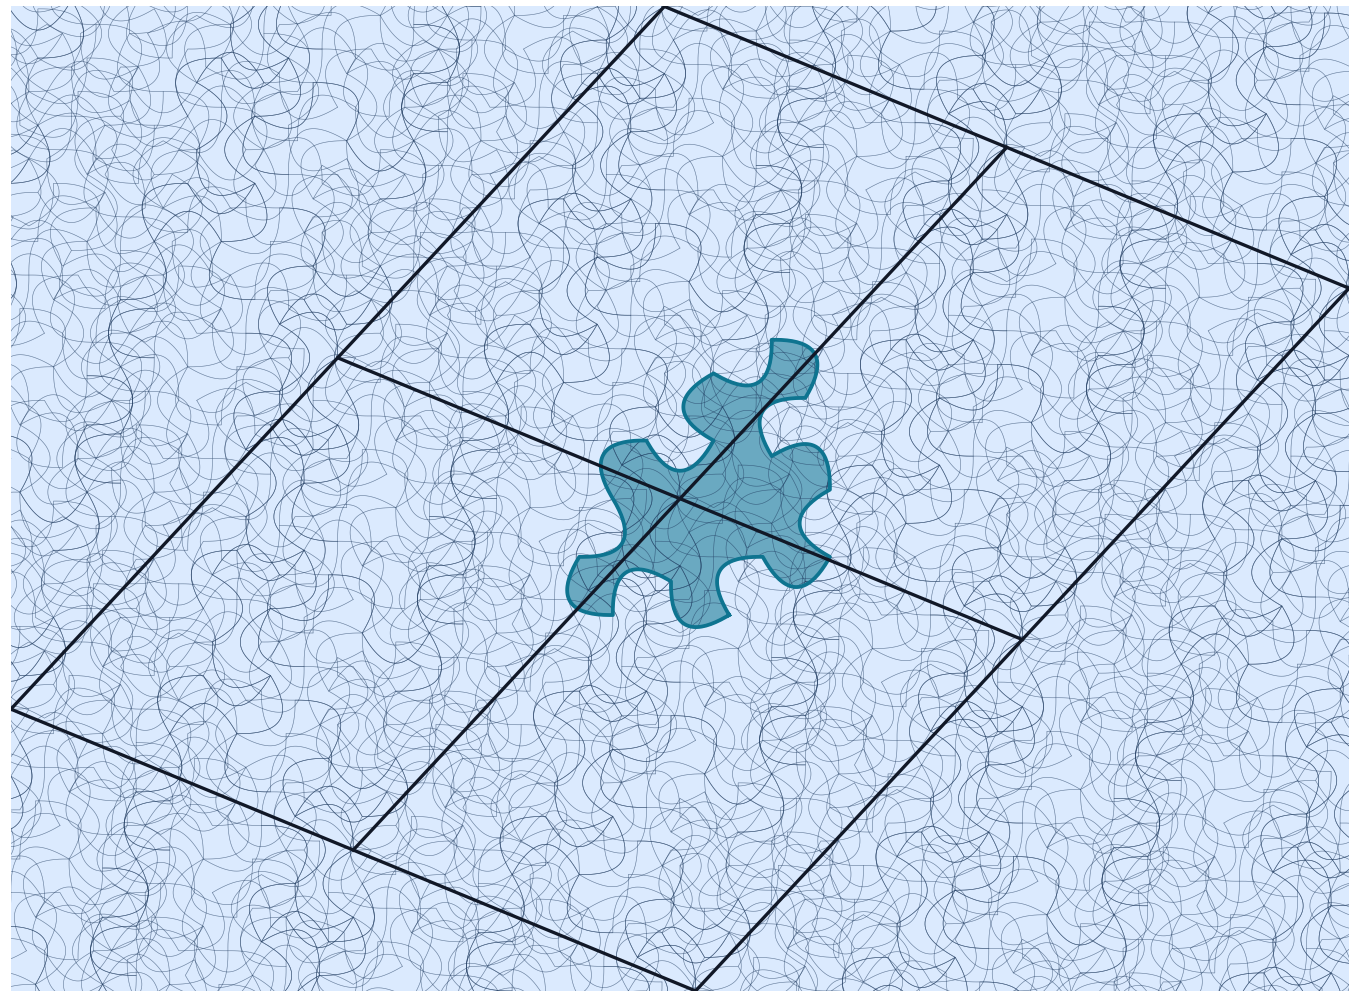
\includegraphics[width=0.82\textwidth]{coverage_map.png}
\caption{Four period cells (black lines) of the cover by a curved Spectre, with one tile shaded. Every one of
the $359{,}800$ sample points of the grid lies in exactly $12$ tiles.}\label{fig:cover}
\end{figure}

\begin{remark}
The construction was found by a computer search for a set of placements whose edge records cancel. Such a
cancellation forces a constant covering number on its own, which is why no matching rules or local
configurations of Spectre tilings enter the argument.
\end{remark}

\section{Formal verification}\label{sec:lean}

For the straight-edged Spectre, Theorem~\ref{thm:main} is proved in Lean~4 with Mathlib~\cite{mathlib}: for
the $54$ placements and every vector of $\Lambda$, almost every point of the plane lies in exactly $12$
tiles. The proof triangulates the tile, shows in general that a periodic family of triangles whose edges
cancel modulo the lattice has an almost everywhere constant count, and computes the constant from the areas.
The finite facts (the cancellation of the $1944$ triangle edges, the orientation of every triangle, the
triangulation's boundary, the distinctness of the placements) are checked by the kernel, and the curved-edge
records of Lemma~\ref{lem:pairs} are checked the same way. The step from those records to constant coverage
for a curved Spectre, which needs the Jordan curve theorem, is not formalised. Everything uses only Lean's
standard axioms, and planted errors in the statements are rejected. A program checks the records and the
areas in exact integer arithmetic, an independent one counts the tiles at random points, and the code and the
Lean files are at~\cite{repo}.

\section*{Acknowledgements}
The question is Andrew Bayly's. The construction and the record-cancellation certificate were found with
OpenAI Codex, and the Lean formalisation, the independent checks and this text were written with Claude
Opus~5.5 (Anthropic), under the author's direction. The author is responsible for the content of this
preprint, which has not yet been independently reviewed.

\begin{thebibliography}{9}
\bibitem{MO} A.~Bayly, \emph{Can the Spectre form a periodic $n$-fold multi-tiling of the plane for any
integer $n\ge1$?}, MathOverflow question 516016 (2026), \url{https://mathoverflow.net/q/516016}.

\bibitem{GRS} N.~Gravin, S.~Robins and D.~Shiryaev, Translational tilings by a polytope, with multiplicity,
\emph{Combinatorica} 32 (2012) 629--649. doi:10.1007/s00493-012-2860-3.

\bibitem{GT} R.~Greenfeld and T.~Tao, Some variants of the periodic tiling conjecture, arXiv:2505.06757
(2025).

\bibitem{repo} V.~Jandhyala, A periodic twelve-fold tiling by the Spectre: code and Lean proofs,
\url{https://github.com/jvvk/mathematics/tree/main/spectre-twelve-fold}.

\bibitem{Kol} M.~N.~Kolountzakis, On the structure of multiple translational tilings by polygonal regions,
\emph{Discrete Comput. Geom.} 23 (2000) 537--553. doi:10.1007/s004540010014.

\bibitem{mathlib} The mathlib Community, The Lean mathematical library, in \emph{Proceedings of the 9th ACM
SIGPLAN International Conference on Certified Programs and Proofs (CPP 2020)}, ACM, 2020, 367--381.
doi:10.1145/3372885.3373824.

\bibitem{SMKG} D.~Smith, J.~S.~Myers, C.~S.~Kaplan and C.~Goodman-Strauss, A chiral aperiodic monotile,
\emph{Combinatorial Theory} 4(2) (2024). doi:10.5070/C64264241.
\end{thebibliography}
\end{document}
